\documentclass[]{article}
\usepackage{lmodern}
\usepackage{amssymb,amsmath}
\usepackage{ifxetex,ifluatex}
\usepackage{fixltx2e} % provides \textsubscript
\ifnum 0\ifxetex 1\fi\ifluatex 1\fi=0 % if pdftex
  \usepackage[T1]{fontenc}
  \usepackage[utf8]{inputenc}
\else % if luatex or xelatex
  \ifxetex
    \usepackage{mathspec}
    \usepackage{xltxtra,xunicode}
  \else
    \usepackage{fontspec}
  \fi
  \defaultfontfeatures{Mapping=tex-text,Scale=MatchLowercase}
  \newcommand{\euro}{€}
\fi
% use upquote if available, for straight quotes in verbatim environments
\IfFileExists{upquote.sty}{\usepackage{upquote}}{}
% use microtype if available
\IfFileExists{microtype.sty}{%
\usepackage{microtype}
\UseMicrotypeSet[protrusion]{basicmath} % disable protrusion for tt fonts
}{}
\usepackage[margin=1.5in]{geometry}
\usepackage{graphicx}
\makeatletter
\def\maxwidth{\ifdim\Gin@nat@width>\linewidth\linewidth\else\Gin@nat@width\fi}
\def\maxheight{\ifdim\Gin@nat@height>\textheight\textheight\else\Gin@nat@height\fi}
\makeatother
% Scale images if necessary, so that they will not overflow the page
% margins by default, and it is still possible to overwrite the defaults
% using explicit options in \includegraphics[width, height, ...]{}
\setkeys{Gin}{width=\maxwidth,height=\maxheight,keepaspectratio}
\ifxetex
  \usepackage[setpagesize=false, % page size defined by xetex
              unicode=false, % unicode breaks when used with xetex
              xetex]{hyperref}
\else
  \usepackage[unicode=true]{hyperref}
\fi
\hypersetup{breaklinks=true,
            bookmarks=true,
            pdfauthor={Daniel W. Hill, Nils W. Metternich, Andreas Beger, and Michael D. Ward},
            pdftitle={Splitting it up: A split-duration package},
            colorlinks=true,
            citecolor=blue,
            urlcolor=blue,
            linkcolor=magenta,
            pdfborder={0 0 0}}
\urlstyle{same}  % don't use monospace font for urls
\setlength{\parindent}{0pt}
\setlength{\parskip}{6pt plus 2pt minus 1pt}
\setlength{\emergencystretch}{3em}  % prevent overfull lines
\setcounter{secnumdepth}{0}

%%% Use protect on footnotes to avoid problems with footnotes in titles
\let\rmarkdownfootnote\footnote%
\def\footnote{\protect\rmarkdownfootnote}

%%% Change title format to be more compact
\usepackage{titling}

% Create subtitle command for use in maketitle
\newcommand{\subtitle}[1]{
  \posttitle{
    \begin{center}\large#1\end{center}
    }
}

\setlength{\droptitle}{-2em}
  \title{Splitting it up: A split-duration package}
  \pretitle{\vspace{\droptitle}\centering\huge}
  \posttitle{\par}
  \author{Daniel W. Hill, Nils W. Metternich, Andreas Beger, and Michael D. Ward}
  \preauthor{\centering\large\emph}
  \postauthor{\par}
  \predate{\centering\large\emph}
  \postdate{\par}
  \date{June 8, 2015}



\begin{document}

\maketitle


\begin{abstract}
We present an implementation of split-population duration regression in the \texttt{spduration} R package and an application to data on military coups. The statistical model accounts for units that are immune to a certain outcome and not part of the duration process the researcher is primarily interested in. We provide insights that if immune units exist, we can significantly increase the predictive performance compared to standard duration model. The package includes estimation and forecasting methods for split-population Weibull and Loglogistic models.
\end{abstract}

\section{Introduction}\label{introduction}

Duration models are an important class of statistical estimators that
take into account the duration dependency of outcomes we are interested
in. For example, the risk of dying is not independent of time. Newborns
are at a great risk of dying, but as they grow older this risk declines
and then gradually starts to increase again after the age of 9-10. This
risk can be increased or decreased by behavioral (smoking, exercise,
diet, etc) and structural factors (health care, regulations, urban vs
rural, etc), but there is an underlying risk that is time dependent and
impacts on all units.

However, sometimes we are interested in situations in which not all
units are at risk of dying, failing, or acquiring some new
characteristic. Imagine we are interested in the risk of acquiring the
flu. First, we might think that everyone is at risk of getting the flu
and it just depends on individual behavior (e.g.~good hygiene) and
structural factors (e.g.~workplace) whether individuals will acquire the
flu. If this would be the case we could use a standard duration model
and estimate how different factors impact on the baseline risk. But
there might also be individuals who are immune to the flu, because they
received a flu shot, had the same flu virus in the past year, or some
other factors that makes it impossible for them to get sick. Given that
this is the case we have two underlying populations: An at risk
population and an immune one. If the immune population is relatively
large, estimates using a standard duration model will be biased and
predictions resulting from such a model inaccurate.

\section{Immune populations and inference of duration
processes}\label{immune-populations-and-inference-of-duration-processes}

Duration models, where the variable to be modeled describes a
distribution of times until some event of interest, were originally
developed in health and demographic research, where they grew naturally
from life tables and survival records for medical patients. Basic
formulations of such models, like the parametric exponential or Weibull
regressions or semi-paramaetric Cox regression, implicitly assume that
all subjects or units under observation, including right-censored
observations, will eventually experience the event of interest. This
assumption is outright wrong or at least disadvantageous in many
substantive areas and empirical applications, where there instead is a
sub-population of units or subjects that will never experience an event,
and thus are effectively ``cured''.

This insight was realized as early as 1949 by Boag (1949) and Berkson
and Gage (1952), who were researching survival rates in cancer patients
following treatment, and where quite obviously some fraction of patients
survived because their cancer was cured, while others relapsed after
apparent remission due to levels of disease below detectable thresholds.
As with conventional duration models, their origin in health and
medicine has shaped the terminology conventionally used with such model,
e.g.~split-population duration models are sometimes also referred to in
such contexts as cure rate models, and the basic concepts like survival
and failure rates reference the survival of humans.

Yet the intuition underlying split-population duration models has led to
applications in a broad range of subject areas outside demographics and
medicine. In an early and foundational application that reached beyond
criminal science, Schmidt and Witte (1989) examined criminal recidivism
using data on close to 10,000 prisoners from the North Carolina prison
system in the late 1970's and early 1980's to identify factors that
influence whether a criminal lapses at all, and if so which factors are
related to the amount of time between prison stints. This work already
includes a full formulation of the model with independent covariates for
both the duration equation and the risk or cure equation, although only
with subject-specific covariates rather than time-varying covariates
with multiple data points per subject.

In public health, Douglas and Hariharan (1994) use data from the US to
model factors related to the age at which smokers started the habit, and
Forster and Jones (2001) examines the impact of tobacco taxes on smoking
and quitting decisions. DeYoung (2003) models the failure of new
commercial banks in the US during the 1980's. Lastly, in our own domain,
political science, Svolik (2008) used a split-population duration
framework to study democratic consolidation, i.e.~whether democratic
regimes persist or slide back to authoritarianism, and when. Building on
this effort, split-population duration models have also been used, along
with other models, to produce regular predictions for five different
forms of political conflict for the Integrated Crisis and Early Warning
System (ICEWS) project (M. D. Ward et al. 2013) and to model irregular
leadership changes for the Political Instability Task Force (PITF;
Beger, Dorff, and Ward 2014).

\section{Model development}\label{model-development}

Conventional duration models assume that all subjects will eventually
fail, if we can only observe them long enough. The likelihood for a data
point with survival time \(t\) is thus the failure rate at that time or
the probability of survival beyond \(t\), depending on whether the
observation is right-censored (\(1-\delta_i\)) or not:

\begin{eqnarray}
\mathcal{L} = \prod_{i=1}^N  \left( f(t_i)\right)^{\delta_i} \times \left( S(t_i) \right)^{1-\delta_i}
\end{eqnarray}

The major modeling question in this setting, which we will return to
below, is the choice of a function to describe the evolution of the
hazard rate \(h(t) = \frac{f(t)}{S(t)}\) over time, e.g.~with
exponential, Weibull, or log-logistic densities.

The cumulative failure rate (\(F(t) = 1 - S(t)\)) over time converges to
1, meaning all subjects fail eventually. This assumption is untenable in
many situations. Some cancer patients are cured after treatment while
others relapse, most young people do not start smoking even though most
smokers started at a young age, and many states will not experience the
kind of violence that persists in some parts of the world. A better
assumption in such contexts is that there is a subpopulation of subjects
who are at risk of experiencing an event at some point, and another
subpopulation who will never experience the event.

The presence of a large sub-population which is not at risk for an event
in practice will inflate estimates of the survival fraction, and reduce
hazard estimates for all subjects by essentially, and falsely,
distributing risk among subjects that genuinely will fail and those that
are cured. A model will thus over predict hazard for subjects that are
not at risk (cured), and under predict for those who are at risk of
eventually experiencing the event of interest.

We can incorporate the presence of a sub-population, where we label the
subpopulation at risk with \(\pi\), by rewriting the likelihood
as:\footnote{Usual presentation of the split-population duration framework in medical contexts focus on the ``cured'' subpopulation. In our applications events are typically rare and it thus is easier to emphasize the ``risk'' subpopulation. As risk $= 1 - $ cured, this difference is trivial.}

\begin{align}
\mathcal{L}\{\theta|(t_{1}, \dots, t_{n})\} &= \prod_{i=1}^{N} \left(\pi_i f(t_i)\right)^{\delta_i} \times  \left((1-\pi_i) + \pi_i S(t_i)\right)^{1-\delta_i}
\end{align}

Crucially, this split-population framework is primarily useful in
contexts where sub-populations are not clearly or easily identifiable.
Even though there is a clear sub-populations in a model of the age at
first pregnancy for humans---men---no researcher in their right mind
would think to include male subjects in their data at all, for example.
On the other hand, whether a cancer patient is cured or not cured given
that they have no visible signs of cancer following treatment or have
hit the 5-year disease free survival mark is much less clear and in fact
the question that initially led to the idea for split-population
duration modeling (Boag 1949, Berkson and Gage (1952)).

Early efforts focused only on the cure rate (\(1 - \pi\)) and treated it
as a constant, but we can model membership in the subpopulation with its
own covariates through a logistic link function:

\begin{align}
\pi_i &= \frac{1}{1 + e^{-z_i \gamma}}
\end{align}

Where \(z_i\) is a vector of covariates for a subject at a given time.
For interpretation, it is important to note that with time-varying
covariates, the risk (or cured) estimate for a subject is particular to
a given time point rather than constant for that subject over all time
periods in the
spell.\footnote{We use ``spell'' to designate all time periods observed for a subject up to the failure time. Subjects can theoretically have multiple spells, e.g. cancer patients who go into remission and relapse more than once, or states that experience multiple civil war onsets over their history.}
Depending on the covariates, the risk estimate for a subject can thus
fluctuate rapidly over time. To ease interpretation, it might be
convenient to restrict covariates in the logit risk model to
slow-moving, stable covariates in order to produce stable risk estimates
for subjects.

The last component to complete the likelihood is the choice of a
distribution for the shape of the hazard rate. The \texttt{spduration}
package implements two hazard rate shapes,
Weibull\footnote{In the code, $f(t) = \alpha \lambda^{\alpha} t^{\alpha - 1} e^{-(\lambda t)^\alpha}$.}
and log-logistic:

\begin{eqnarray*}
\textrm{Weibull} \\
 f(t) & = & \alpha \lambda (\lambda t)^{\alpha - 1} e^{-(\lambda t)^\alpha} \\
  S(t) & = & e^{ -(\lambda t )^\alpha } \\
 h(t) & = & \alpha \lambda (\lambda t)^{\alpha-1} \\
\textrm{Log-logistic} \\
 f(t) & = & \frac{ \alpha \lambda (\lambda t)^{\alpha-1} }{ (1 + (\lambda t)^\alpha)^2 } \\
 S(t) & = & \frac{1}{ 1+  (\lambda t)^\alpha }  \\
 h(t) & = & \frac{ \alpha \lambda (\lambda t)^{\alpha-1} }{ 1+  (\lambda t)^\alpha }
\end{eqnarray*}

Where \(\lambda = e^{-x_i\beta}\) is a parameter of covariates.

With these, the main quantity of interest is the conditional hazard
\(h(t, \pi)\), where both the risk/cure probabilities and hazard are
conditional on survival to time \(t\):

\begin{eqnarray}
h(t, \pi) = \frac{f(t, \pi)}{S(t, \pi)} & = & \frac{ \pi(t) \times f(t) }{ (1-\pi(t)) + \pi(t) \times S(t) } \\
 \pi(t) & = & \frac{ 1-\pi }{ S(t) + (1-\pi) (1 - S(t)) }
\end{eqnarray}

For a given unconditional risk rate \(\pi\), the probability that a
particular case with survival time \(t\) is in the risk set decreases
over time because an increasing number of surviving cases consist of
immune or cured (\(1-\pi\)) cases that will never fail. In the hazard
rate, the failure rate in the numerator is conditional on the
probability that a case is in the risk set, give survival up to time
\(t\), and the numerator is an adjusted survivor function that accounts
for the fraction of cured cases by time \(t\), which is \(1-\pi(t)\).

\section{Fit a split-population model on coups
data}\label{fit-a-split-population-model-on-coups-data}

The \texttt{spduration} package implements a split-population duration
regression for data with time-varying covariates and with two options
for the hazard rate shape, the Weibull and
log-logistic.\footnote{The Weibull allows for monotonically increasing or decreasing hazard rates, while the log-logistic allows for rates that first increase and then decrease.}
The primary function, \texttt{spdur}, produces a regression model object
of class \texttt{spdur} which can then be used with further methods.

To illustrate the usefulness of the package and the broad applicability
of the methods outlined above, we employ an example from political
science. We replicate and extend the analysis presented in Belkin and
Schofer (2003), which examines factors that lead to military coups.
Belkin and Schofer's distinction between ``structural'' vs.
``triggering''" causes of coups strongly suggests that a
split-population approach to this question will be useful. They argue
that many countries never experience coups because coups are effectvely
impossible due to structural factors, while others that never experience
coups are nevertheless at risk due to a different configuration of those
same factors. Using language which fits nicely with the class of models
described above, they say ``Triggers are not the source of the original
risk, and in the absence of structural causes, the presence of
triggering factors alone cannot lead to a coup. Hence, triggers should
not be equated with coup risk. Rather, they are factors that may
determine the exact timing of a coup in regimes that suffer from high
coup risk'' (p.~598 Belkin and Schofer 2003). Belkin and Schofer develop
a measure of ``structural coup risk'' which incorporates factors such as
the strength of democratic institutions and civil society, and a recent
history of successful coups. They employ a logistic regression model
which does not adequately capture the process described in the quote
above, since it implicitly assumes that all observations are at risk for
a coup (i.e., the probability of a coup is non-zero for all
observations). Their structural coup risk indicator is developed
precisely to distinguish between cases where coups are possible and
cases where they are not, so the split-population model allows one to
examine whether the indicator effectively separates at-risk cases from
cases where coups are impossible.

We begin by loading the package and formatting the data appropriately.
\small

\begin{verbatim}
> library(spduration)
> new.coup.data <- add_duration(coup.data, "coup", unitID="countryid", tID="year", 
+   freq="year")
\end{verbatim}

\normalsize
The \texttt{add}\_\texttt{duration} function takes as input a data frame
with a binary response variable (in this example, ``coup''``) that
measures the occurrence of the event, or failure, recorded over discrete
time periods, and produces a data frame with a duration variable
(named''duration``) for each spell as well as a binary variable
(''atrisk``) that is constant across the spell and indicates whether the
spell ended in failure. These are then used as response variables for
the formula in the \texttt{spdur} function. Though the data used in this
example are recorded annually, the function supports annual, monthly, or
daily data. We begin by fitting first a Weibull and then a log-logistic
split-population duration model using the coups data, including the
measure of coup risk in the logit (risk) equation. \small

\begin{verbatim}
> weib.model <- spdur(duration~Military.Regime+Instability+Recent.War+Regional.Conflict,
+       atrisk~Coup.Risk+GDP.cap.+Military.Regime+
+       Recent.War+Regional.Conflict+
+       South.Am.+Central.Am.,data=new.coup.data)
> loglog.model <- spdur(duration~Military.Regime+Instability+Recent.War+Regional.Conflict,
+       atrisk~Coup.Risk+GDP.cap.+Military.Regime+
+       Recent.War+Regional.Conflict+
+       South.Am.+Central.Am.,data=new.coup.data,distr="loglog")
\end{verbatim}

\normalsize  
Using the \texttt{summary} function on either model object will produce
standard output showing the model formula, estimates for the duration
and risk equations, and test statistics with \(p\)-values. One may also
use the \texttt{AIC} and \texttt{BIC} function to calculate the
information criterion statistics for \texttt{spdur} objects.\\\small

\begin{verbatim}
> AIC(weib.model)
[1] 1120.774
> AIC(loglog.model)
[1] 1111.908
> BIC(weib.model)
[1] 1209.577
> BIC(loglog.model)
[1] 1200.711
\end{verbatim}

\normalsize
The objects produced by \texttt{spdur} can also be used with functions
in the \texttt{xtable} package to produce \LaTeX~code for tables of
results. The \texttt{xtable} function used on an \texttt{spdur} object
will produce code such as that used to create Table \ref{loglog_table}.
\small

\begin{verbatim}
> xtable(loglog.model,caption="Coup model with log-logistic hazard")
\end{verbatim}

\begin{table}[ht]
\centering
\caption{Coup model with log-logistic hazard} \label{loglog_table}
\begin{tabular}{rlrrr}
  \hline
 & Parameter & Estimate & StdErr & p \\ 
  \hline
1 & (Dur. Intercept) & 3.29 & 0.14 & 0.00 \\ 
  2 & Military.Regime & -1.51 & 0.16 & 0.00 \\ 
  3 & Instability & -0.21 & 0.04 & 0.00 \\ 
  4 & Recent.War & -0.20 & 0.28 & 0.48 \\ 
  5 & Regional.Conflict & 2.64 & 2.56 & 0.30 \\ 
  6 & log(alpha) & -0.53 & 0.07 & 0.00 \\ 
  7 & (Risk Intercept) & -13.10 & 10.03 & 0.19 \\ 
  8 & Coup.Risk & 7.32 & 3.23 & 0.02 \\ 
  9 & GDP.cap. & 3.11 & 1.82 & 0.09 \\ 
  10 & Military.Regime.1 & 25.41 & 0.01 & 0.00 \\ 
  11 & Recent.War.1 & -4.34 & 2.70 & 0.11 \\ 
  12 & Regional.Conflict.1 & -39.74 & 23.96 & 0.10 \\ 
  13 & South.Am. & -3.72 & 3.19 & 0.24 \\ 
  14 & Central.Am. & -6.08 & 2.45 & 0.01 \\ 
   \hline
\end{tabular}
\end{table}

\normalsize
The table shows estimates from the duration equation, beginning with the
intercept, and then estimates from the risk equation. Interestingly, the
coup risk variable has a rather large and statistically significant
coefficient in the risk equation.

The package also includes a function, \texttt{plot.hazard}, that can be
used with an \texttt{spdur} object to plot the estimated hazard rate.
\texttt{plot.hazard} plots the conditional hazard, which is the
probability of survival conditional on the covariates in the risk and
duration equations, and conditional on survival up to time \(t\). The
function calculates the estimated hazard rate as well as 90\% confidence
intervals, which are produced by simulating values from the estimated
sampling distributions of the model parameters. By default the function
uses the mean values of the covariates during the simulations, but users
can choose specific covariate values by entering them as vectors in the
arguments \texttt{xvals} and \texttt{zvals}, which correspond to the
covariates in the duration and risk equations, respectively. The command
below creates Figure \ref{hazard}.

\begin{verbatim}
> plot.hazard(loglog.model)
\end{verbatim}

\begin{figure}[htbp!]
\centering
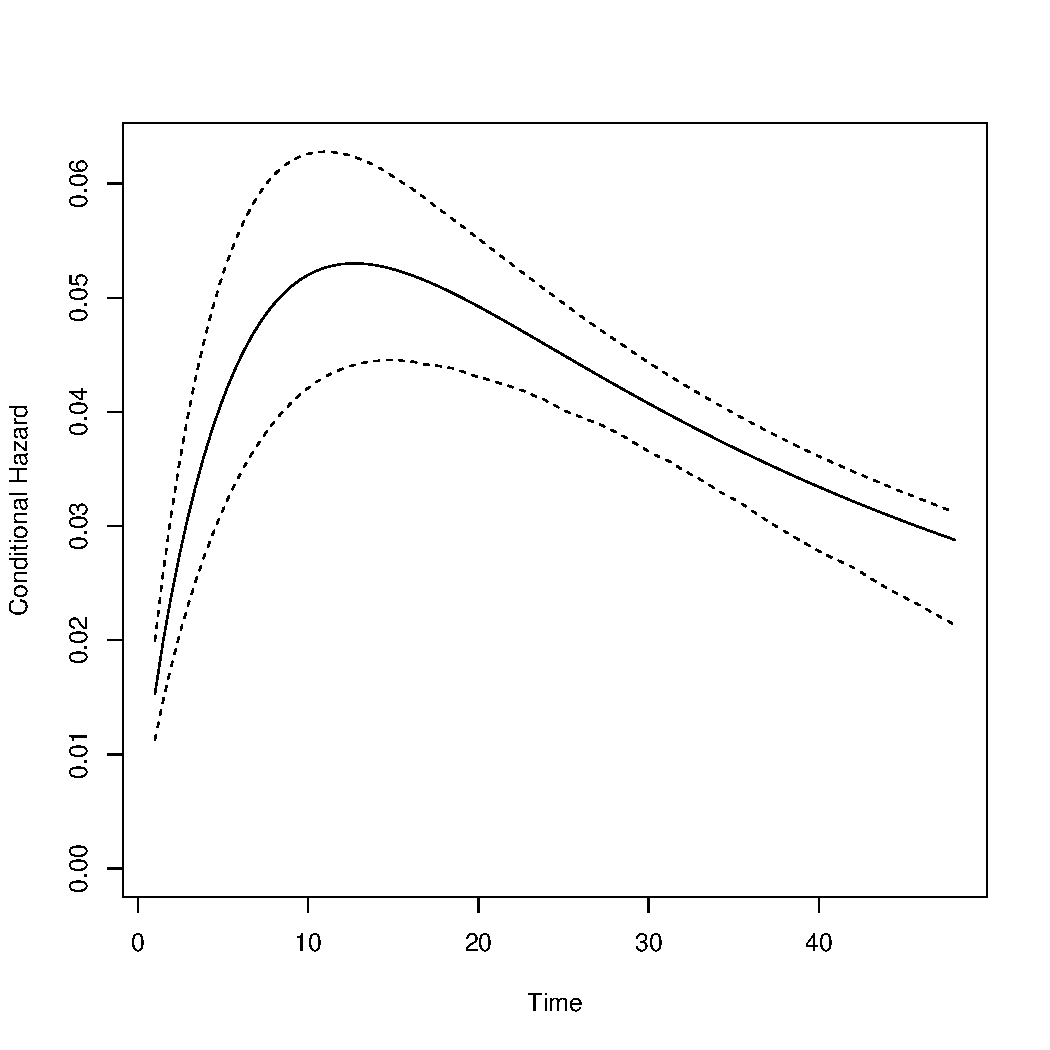
\includegraphics[width=4in]{loglog_hazard.pdf}
\caption{Conditional hazard rate from log-logistic model.} \label{hazard}
\end{figure}

Importantly, the package also includes functions to evaluate model
predictions. The generic function \texttt{predict} can be used on an
object of class \texttt{spdur} to generate several kinds of predictions,
including the probability that an observation is ``at-risk'' and the
probability of failure for a given time period. In addition, the generic
\texttt{plot} function can be used on \texttt{spdur} objects to produce
a separation plot (Greenhill, Ward, and Sacks 2011), which is a
graphical display for evaluating model predictions. The code below
produces Figure \ref{insamp}. \small

\begin{verbatim}
> dev.new(width=9,height=3)
> par(mfrow=c(2,1),mar=c(2,2,2,2))
> plot(weib.model,endSpellOnly=F)
> plot(loglog.model,endSpellOnly=F)
\end{verbatim}

\normalsize
The option \texttt{endSpellOnly} is set to \texttt{FALSE} so that every
observation, not only those at the end of a spell, is used in the plot.
By default the \texttt{plot} function will calculate the conditional
hazard for each observation. The separation plot sorts observations from
left to right according to the predicted probability assigned by the
model (higher values to the right), and shows each event/failure as red
line, with non-events shown in beige. This makes it easy to see whether
the model is assigning high probabilities of failure to actual cases of
failure, and low probabilities to non-failures.

\begin{figure}[htbp!]
\centering
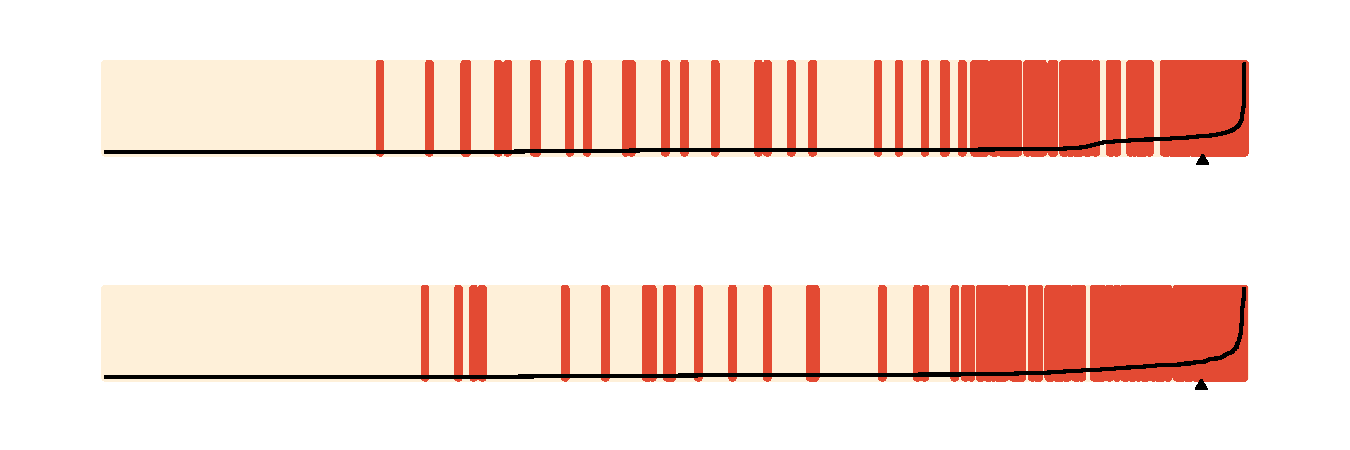
\includegraphics[width=5in]{in-sample.pdf}
\caption{{\em In-sample separation plots for Weibull and log-logistic models.}} \label{insamp}
\end{figure}

Finally, we demonstrate use of the \texttt{spdurCrisp} function for
evaluating out-of-sample predictions. We begin by splitting the data
into training and test sets, using the last year of data (1999) as the
test set and omitting incomplete observations from the test set. \small

\begin{verbatim}
> coup.train<-new.coup.data[coup.data$year<1999,]
> coup.test<-new.coup.data[new.coup.data$year==1999,]
> coup.test<-na.omit(coup.test)
\end{verbatim}

\normalsize
The \texttt{spdurCrisp} function can then be used to fit a model on the
training set and generate predictions for the test set. \small

\begin{verbatim}
> weib.model2<-spdurCrisp(duration~Military.Regime+Instability+Recent.War+Regional.Conflict,
+       atrisk~Coup.Risk+GDP.cap.+Military.Regime+Recent.War+Regional.Conflict+
+       South.Am.+Central.Am.,
+       last='end.spell',train=coup.train,test=coup.test,pred=coup.test)
> weib.preds<-as.numeric(weib.model2$test.p)
>
> loglog.model2<-spdurCrisp(duration~Military.Regime+Instability+Recent.War+Regional.Conflict,
+       atrisk~Coup.Risk+GDP.cap.+Military.Regime+Recent.War+Regional.Conflict+
+       South.Am.,
+       last='end.spell',train=coup.train,test=coup.test,pred=coup.test,distr="loglog")
> loglog.preds<-as.numeric(loglog.model2$test.p)
\end{verbatim}

\normalsize
The \texttt{train},\texttt{test}, and \texttt{pred} arguments are used
to specify data frames for the training set, test set, and forecasting
set. We do not wish to generate forecasts here, so we simply specify the
same data frame for the test and forecasting set. Here we use
\texttt{spdurCrisp} to calculate the conditional risk, which is the
default calculation for this function and is the probability that an
observation is in the at-risk population. The test set predictions are
stored in the model object as \texttt{test.p}, and we extract them to
produce the plot shown below in Figure \ref{outsamp}, which was created
using the \texttt{separationplot} package. \small

\begin{verbatim}
> dev.new(width=9,height=3)
> par(mfrow=c(2,1),mar=c(2,2,2,2))
> separationplot(weib.preds,coup.test$Coup,newplot=F,show.expected=T,lwd1=5,lwd2=2)
> separationplot(loglog.preds,coup.test$Coup,newplot=F,show.expected=T,lwd1=5,lwd2=2)
\end{verbatim}

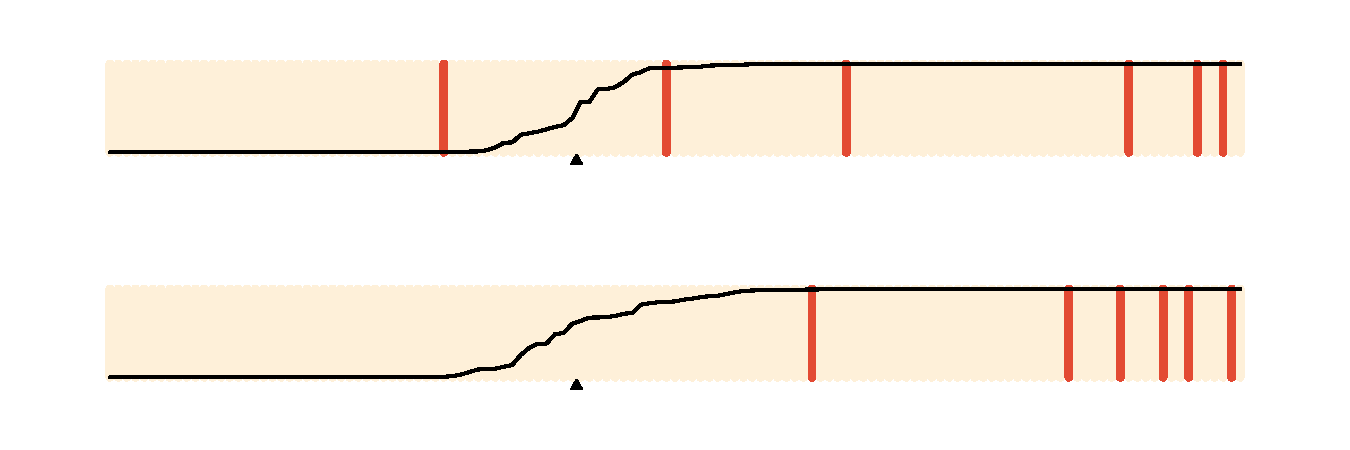
\includegraphics{out-of-sample.pdf}

\normalsize

\begin{figure}[htbp!]
\centering
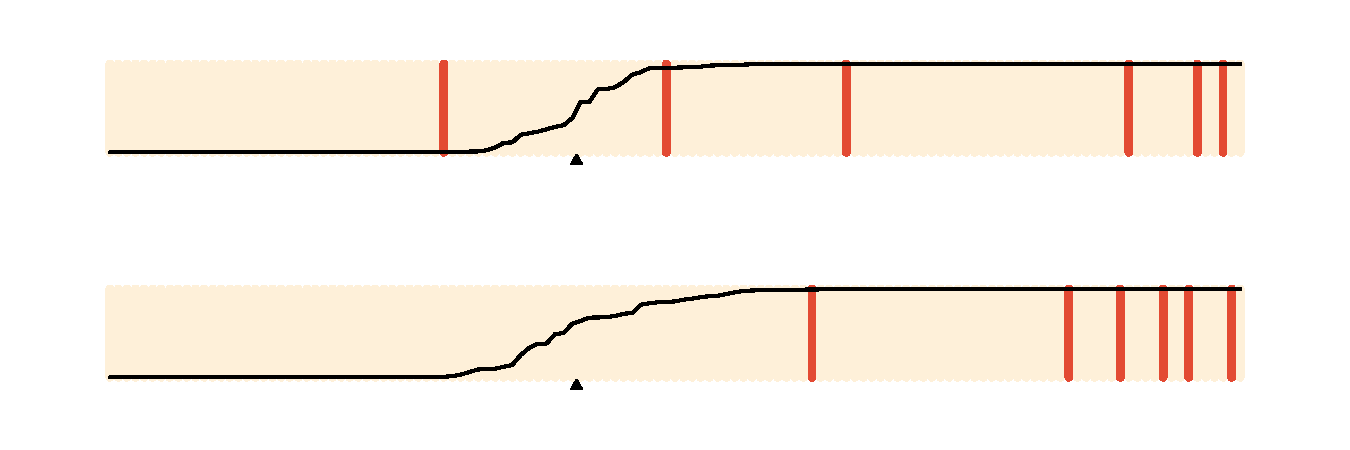
\includegraphics[width=5in]{out-of-sample.pdf}
\caption{{\em Out-of-sample separation plots for Weibull and log-logistic models. }} \label{outsamp}
\end{figure}

\section{Censoring considerations}

Truncation and censoring are problematic for split-population duration
models as they are for standard duration regression, but also pose some
additional considerations. In left-truncation, we do not observe data
for a spell prior to some date, and thus have incomplete and inaccurate
values for the duration or time to failure for a spell. Since immune
spells in the sample are over time going to distinguish themselves with
exceptionally long survival times compared to spells at risk which fail
periodically, left-censoring also makes it more difficult to distinguish
the immune and at risk subpopulations.

Sometimes information about previous failures in the data is available
beyond the time period over which covariates are observed, making it
possible to ameliorate or eliminate left-censoring by using the
information of previous failures when constructing the necessary
duration variables with \texttt{add\_duration()}.

Right-censoring, where spells end before outcomes are observed, also
pose a unique problem in the split-population framework. Although
right-censored spells themselves are accommodated in the modeling
function, they impact the coding of at risk vs.~immune spells. The
\texttt{add\_duration()} function retroactively codes all observations
in a spell as at risk if the spell itself ended in failure.
Right-censored spells are coded as immune over their entire duration.
This can lead to some misclassification of observations as immune even
though they experience failure at some point in the unobserved future.

Furthermore, in out-of-sample testing based on some kind of data
partitioning scheme, this coding scheme can lead to unintentioned
contamination of in-sample cases with knowledge of out-of-sample
failures through the risk coding for failed spells. This leads to two
recommendations. First, the duration data (\texttt{add\_duration})
should not be built until after partitioning the data. Secondly, and as
a result of the first point, data should be partitioned in a scheme that
samples either by spell or block-wise, e.g.~by witholding the last
\textbf{x} years of data, in order to be able to proberly build the
duration variables.

\section{Conclusion}\label{conclusion}

\begin{figure}[htbp!]
\centering
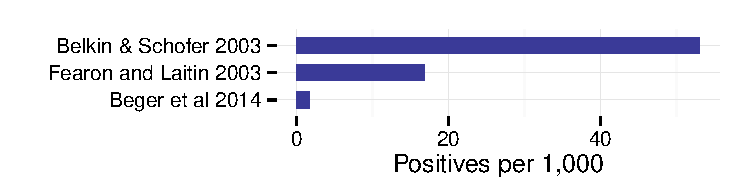
\includegraphics[width = 4in]{graphics/rates.pdf}
\caption{Rates of positive outcomes in select publications with binary outcomes}
\label{rates}
\end{figure}

Data and outcomes in international relations, and to a lesser extent in
other fields as well, are typically characterized by temporal dependence
and, where a binary, ordinal, or count outcome is modelled, rare events
or severely imbalanced classes with excessive numbers of zeros. Figure
\ref{rates} shows a few examples for published research that models
binary outcomes.

This is a well-recognized problem and has led to the development or use
of several specialized mixture models like zero-inflated Poisson and
negative binomial regression for count data, and a zero-inflated ordered
probit for ordinal outcomes (Bagozzi et al. 2015). Split-population
duration regression provides another principled solution to the
challenges posed by data in this domain, but, unlike other solutions to
the sparse outcome problem, also addresses underlying temporal dynamics.

In addition to these technical features, split-population duration
models are also appealing in the context of theories or arguments that
explicitly distinguish long-term structural causes from short-term
triggering events, as Belkin and Schofer (2003) and others do, as this
conceptual distinction can be accomodated through the seperate risk and
duration equations.

\section*{References}\label{references}
\addcontentsline{toc}{section}{References}

Bagozzi, Benjamin E, Daniel W Hill, Will H Moore, and Bumba Mukherjee.
2015. ``Modeling Two Types of Peace the Zero-Inflated Ordered Probit
(ZiOP) Model in Conflict Research.'' \emph{Journal of Conflict
Resolution} 59 (4). SAGE Publications: 728--52.

Beger, Andreas, Cassy L. Dorff, and Michael D. Ward. 2014. ``Ensemble
Forecasting of Irregular Leadership Change.'' \emph{Research \&
Politics} 1 (3).

Belkin, Aaron, and Evan Schofer. 2003. ``Toward a Structural
Understanding of Coup Risk.'' \emph{Journal of Conflict Resolution} 47
(5). Sage Publications: 594--620.

Berkson, Joseph, and Robert P Gage. 1952. ``Survival Curve for Cancer
Patients Following Treatment.'' \emph{Journal of the American
Statistical Association} 47 (259). Taylor \& Francis Group: 501--15.

Boag, John W. 1949. ``Maximum Likelihood Estimates of the Proportion of
Patients Cured by Cancer Therapy.'' \emph{Journal of the Royal
Statistical Society. Series B (Methodological)} 11 (1). JSTOR: 15--53.

DeYoung, Robert. 2003. ``The Failure of New Entrants in Commercial
Banking Markets: A Split-Population Duration Analysis.'' \emph{Review of
Financial Economics} 12 (1). Elsevier: 7--33.

Douglas, Stratford, and Govind Hariharan. 1994. ``The Hazard of Starting
Smoking: Estimates from a Split Population Duration Model.''
\emph{Journal of Health Economics} 13 (2). Elsevier: 213--30.

Forster, Martin, and Andrew M Jones. 2001. ``The Role of Tobacco Taxes
in Starting and Quitting Smoking: Duration Analysis of British Data.''
\emph{Journal of the Royal Statistical Society: Series A (Statistics in
Society)} 164 (3). Wiley Online Library: 517--47.

Greenhill, Brian, Michael D Ward, and Audrey Sacks. 2011. ``The
Separation Plot: A New Visual Method for Evaluating the Fit of Binary
Models.'' \emph{American Journal of Political Science} 55 (4). Wiley
Online Library: 991--1002.

Schmidt, Peter, and Ann Dryden Witte. 1989. ``Predicting Criminal
Recidivism Using Split Population Survival Time Models.'' \emph{Journal
of Econometrics} 40 (1). Elsevier: 141--59.

Svolik, Milan. 2008. ``Authoritarian Reversals and Democratic
Consolidation.'' \emph{American Political Science Review} 102 (02).
Cambridge Univ Press: 153--68.

Ward, Michael D, Nils W Metternich, Cassy L Dorff, Max Gallop, Florian M
Hollenbach, Anna Schultz, and Simon Weschle. 2013. ``Learning from the
Past and Stepping into the Future: Toward a New Generation of Conflict
Prediction.'' \emph{International Studies Review} 15 (4). Wiley Online
Library: 473--90.

\end{document}
